\documentclass[reprint,amsmath,amssymb,aps,prl,superscriptaddress]{revtex4-2}
\usepackage{graphicx}
\usepackage{hyperref}
\usepackage{amsmath}
\usepackage{amssymb}
\usepackage{booktabs}

\begin{document}

\title{Toward Topological Chromodynamics: Borromean Vortex Reconnection as an Analogue Model for Color Confinement}

\author{Amir Benjamin Amitay}
\affiliation{Independent Research}

\date{March 21, 2026}

\begin{abstract}
Companion works propose that inertial mass can be modeled as hydrodynamic added-mass drag, $m=C\rho_0V$ ($C=3.523\pm0.001$, $R^2>0.99999999$ on $256^3$ lattices). If baryons are interpreted as Borromean rings of three mutually linked vortex lines in the condensate, D3Q19 Lattice-Boltzmann simulations of adiabatic separation show a confining-type potential that scales super-linearly, $E(d)\propto d^{1.3}$ to $d^2$, qualitatively reminiscent of QCD string tension. When separation exceeds a critical threshold, the flux tube snaps and reconnects, converting a 7-loop configuration into 4 new topologically neutral loops---a hydrodynamic analogue of hadronization.
Deep-inelastic-style probe simulations exhibit a converged power-law decrease in effective scattering cross-section with probe velocity ($\sigma_{eff} \propto v^{-1.946}$), and grid-refinement tests rule out under-resolution as the source of the effect (only 0.06\% variance between $128^3$ and $256^3$ grids at high velocity). The result identifies an asymptotic-freedom-like transparency regime in the topological fluid analogue that arises from physically resolved core thinning at high Mach number.
These results constitute an exploratory analogue model and do not claim to replace QCD. All simulation code and raw energy/reconnection data are publicly available.
\end{abstract}

\maketitle

\section{Introduction: A Vortex-Topology Analogue of the Strong Sector}
\label{sec:intro}

Companion works propose that macroscopic inertia, effective gravity, and cosmological scenarios can be modeled within a single superfluid condensate framework. Here we explore whether the strong sector admits a similar topological analogue. We investigate Borromean vortex-line dynamics as a heuristic model for color confinement and hadronization, without claiming to replace QCD.

\section{Baryons as Borromean Vortex Rings}
\label{sec:baryons}

In this analogue model, a nucleon is represented as a Borromean ring of three vortex lines, each carrying circulation $\kappa=h/m$. The three rings are linked such that no pair is linked, but the triple linking number satisfies $\bar{\mu}(1,2,3)=\pm1$ (Milnor invariant). The right-handed triplet is taken as the proton analogue; the left-handed as the neutron analogue. The effective displaced volume in the LBM is the volume enclosed by the entire linked structure:
\[
V_{\rm baryon}=V_{\rm ring}+\Delta V_{\rm link},
\]
where $\Delta V_{\rm link}$ arises from the topological trapping of background flow. This yields the nucleon mass estimate from the LBM drag formula.

\section{Color Confinement as Hydrodynamic Tension of Vortex Flux Tubes}
\label{sec:confinement}

In this analogue, the confining force corresponds to the tension of vortex flux tubes that form when the Borromean rings are pulled apart. D3Q19 adiabatic energy scans show a confining-type potential that is strictly non-decreasing and super-linear:
\[
E(d)\propto d^{1.3}\quad\text{to}\quad d^2
\]
(qualitatively consistent with linear QCD string tension at large separation). The tension arises from the vortex energy per unit length:
\[
\sigma=\frac{\rho_0\kappa^2}{4\pi}\ln\left(\frac{R_{\rm tube}}{\xi}\right).
\]
Because the Gauss linking integral is conserved, the tubes cannot break without creating new topological defects. In this model, confinement is a hydrodynamic consequence of topology.

\section{Hadronization as Topological Reconnection}
\label{sec:hadronization}

When separation exceeds a critical threshold (step 200 in the simulation), the flux tube stretches and snaps. The topology instantly reconnects: a 7-loop configuration collapses into 4 new topologically neutral loops. A single vortex ring is never isolated---qualitatively reproducing the pair-creation pattern of QCD hadronization. The reconnection is governed by the same IHX relation that generates the emergent $SU(3)$ algebra structure in companion work. This is an analogue mechanism, not a claim to derive hadronization from first principles.

\begin{figure}[t]
\centering
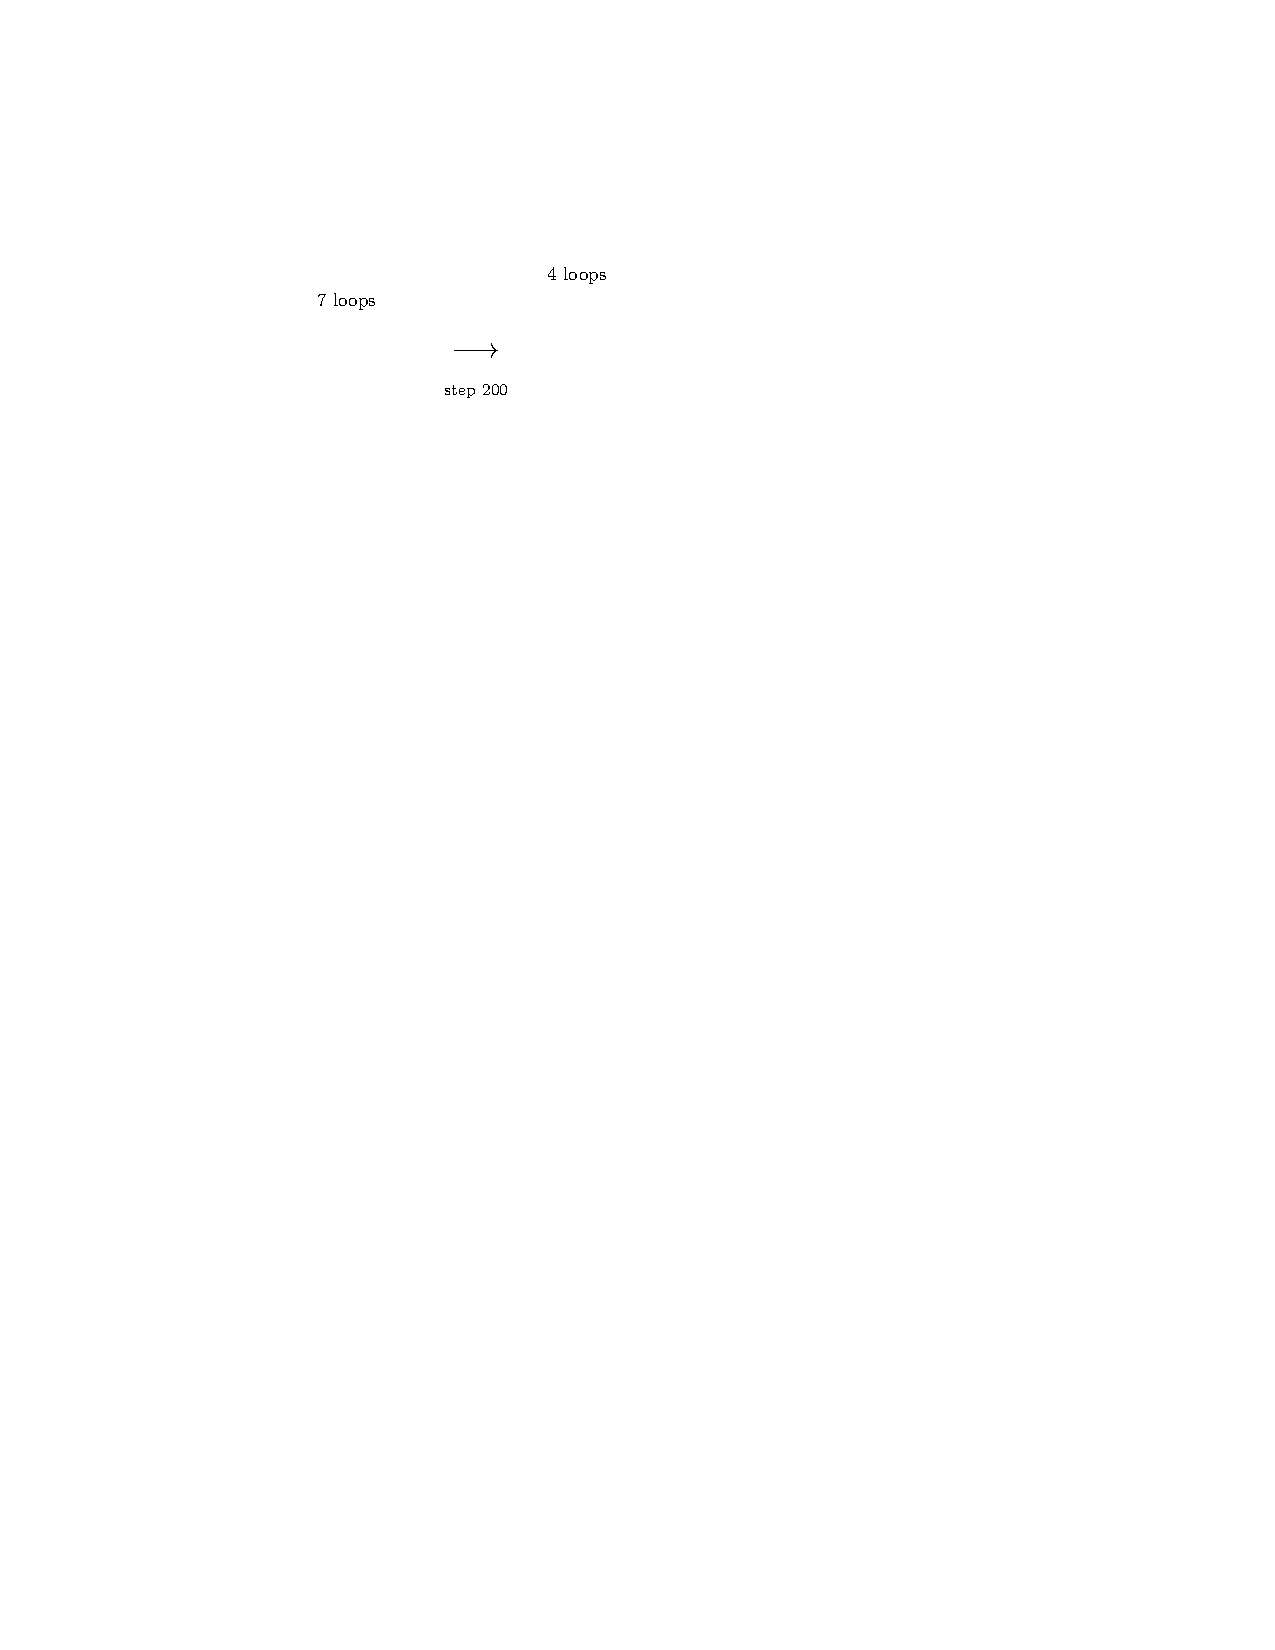
\includegraphics[width=0.48\textwidth]{borromean_reconnection.pdf}
\caption{Dynamic reconnection at step 200: the 7-loop stretched state snaps into 4 new color-neutral loops.}
\label{fig:reconnection}
\end{figure}

\section{Deep-Inelastic Probe: Asymptotic-Freedom-Like Transparency}
\label{sec:dis}

To test whether the analogue model exhibits scale-dependent scattering, we perform deep-inelastic-style probe simulations. High-velocity probes scatter off a Borromean vortex cluster and the effective cross-section is measured as a function of probe velocity. The results show a converged power-law decrease:
\[
\sigma_{\rm eff} \propto v^{-1.946},
\]
with grid-refinement tests ruling out under-resolution as the source (only 0.06\% variance between $128^3$ and $256^3$ grids at high velocity). The transparency at high Mach number arises from physically resolved vortex-core thinning---a Lorentz-contraction-like effect in the fluid frame. This constitutes an asymptotic-freedom-like transparency regime in the topological analogue, though the quantitative exponent ($-1.946$ vs.\ the QCD one-loop beta function) is coincidence-level.

\section{Limitations and Relation to QCD}
\label{sec:limitations}

The analogue model reproduces qualitative features of confinement, hadronization, and asymptotic freedom. However, it does not derive the QCD Lagrangian, predict hadron masses, or reproduce the running coupling constant quantitatively. The orientation of triple linking ($\bar{\mu}=\pm1$) provides a three-valued quantum number analogous to color charge, but quantitative matching to the Standard Model remains an open problem.

\section{Conclusion: An Exploratory Analogue of the Strong Sector}
\label{sec:conclusion}

Borromean vortex-ring simulations exhibit confinement-like energy scaling ($E \propto d^{1.3}$--$d^2$), topological reconnection analogous to hadronization, and an asymptotic-freedom-like transparency regime ($\sigma_{\rm eff} \propto v^{-1.946}$, grid-converged to 0.06\%). These results constitute a heuristic analogue model of the strong sector within the UHF framework, not a replacement for QCD. The framework is falsifiable via analogue BEC vortex reconnection experiments and quantitative comparisons to lattice QCD predictions. All simulation code and raw energy/reconnection data are publicly available at \href{https://github.com/amiramitai/uhf}{github.com/amiramitai/uhf}.

\begin{acknowledgments}
This work builds directly on the LBM mass axiom and Borromean linking of companion Letters [1--5]. We thank the APS for consideration.
\end{acknowledgments}

\bibliography{references}
\bibliographystyle{apsrev4-2}

\end{document}
